% Sprache auswählen!!!
%-> das nicht genutzte auskommentieren
\newif\ifdocenglish
\docenglishtrue % for english
%\docenglishfalse % Für deutsch 


% Klassen-Option language:
\ifdocenglish
  \PassOptionsToClass{language=english}{tudapub}
\else
  \PassOptionsToClass{language=ngerman}{tudapub}
\fi

\documentclass[
	thesis={type=msc}, % Type ändern auf ... sta: Studienarbeit, bsc: Bachelor, msc: Master
%% Die folgenden Parameter sollten nicht geändert werden
	class=report,% Basisdokumentenklasse. Wählt die Korrespondierende KOMA-Script Klasse
	ruledheaders=section,% Ebene bis zu der die Überschriften mit Linien abgetrennt werden, vgl. DEMO-TUDaPub
	accentcolor=1b, % Auswahl der Akzentfarbe
	marginpar=false,% Kopfzeile und Fußzeile erstrecken sich nicht über die Randnotizspalte
	parskip=half-,% Absatzkennzeichnung durch Abstand vgl. KOMA-Script
	fontsize=11pt,% Basisschriftgröße laut Corporate Design ist mit 9pt häufig zu klein
	IMRAD=false, % Zusätzliche Metadaten nach Wunsch der Universitätsbibliothek deaktivieren
%	pdfa=false % tudapub hat einen Workaround für pdfa compilation https://github.com/tudace/tuda_latex_templates/issues/321 Falls kein pdfa notwendig ist: pdfa=false nutzen und das \Metadata Command im Document head entfernen
]{tudapub}

\RedeclareSectionCommand[beforeskip=0pt, afterskip=1.5ex plus .2ex]{chapter}


%%%%%%%%%%%%%%%%%%%
% Sprachanpassung & Verbesserte Trennregeln
%%%%%%%%%%%%%%%%%%%
\ifdocenglish
  \usepackage[main=english, ngerman]{babel}
  \usepackage[english]{datetime2}
\else
  \usepackage[main=ngerman, english]{babel}
  \usepackage[german]{datetime2}
\fi

%\usepackage[ngerman, main=ngerman]{babel} % ngerman und englisch bei deutschen Arbeiten tauschen
%\usepackage[german]{datetime2} % german und english bei der Arbeit anpassen
\usepackage[autostyle]{csquotes} % Anführungszeichen vereinfacht
\usepackage{microtype}
\usepackage[justification=centering]{caption}

%%%%%%%%%%%%%%%%%%%
% Literaturverzeichnis
%%%%%%%%%%%%%%%%%%%

\usepackage[
  backend=biber,
  bibstyle=ieee,        % IEEE-Layout für Einträge
  citestyle=alphabetic, % Textverweise benutzen labelalpha
  sorting=none,
  maxalphanames=1,
  minalphanames=1
]{biblatex}
\addbibresource{Beispielbib.bib}

% Keine automatische Groß-/Kleinschreibung:
\DeclareFieldFormat{titlecase}{#1}
\DeclareFieldFormat{sentencecase}{#1}

\DeclareLabelalphaTemplate{
  \labelelement{\field[strwidth=3,strside=left]{labelname}}
  \labelelement{\field[strwidth=2,strside=right]{year}}
}
\DeclareFieldFormat{labelnumberwidth}{%
  \mkbibbrackets{\printfield{labelalpha}\printfield{extraalpha}}}

% Autoren in Kapitälchen, ohne Doppel-Initialen
\DeclareNameFormat{author}{%
  \nameparts{#1}%
  \textsc{%
    \usebibmacro{name:given-family}
      {\namepartfamily}
      {\namepartgiveni}   % <-- NICHT \namepartgiveni
      {\namepartprefix}
      {\namepartsuffix}%
  }%
  \usebibmacro{name:andothers}%
}

% Links wie normaler Text
\usepackage[hidelinks]{hyperref}
\urlstyle{same}

%%%%%%%%%%%%%%%%%%%
\usepackage{etoolbox}
\usepackage{longtable}
\usepackage{tabularx}
\usepackage[table,xcdraw]{xcolor}
\usepackage{hyperref}
\apptocmd{\UrlBreaks}{\do\f\do\m}{}{}
\setcounter{biburllcpenalty}{9000}% Kleinbuchstaben
\setcounter{biburlucpenalty}{9000}% Großbuchstaben

\DeclareCiteCommand{\footpartcite}[\mkbibfootnote]
    {\usebibmacro{prenote}}
    {%
        \usebibmacro{cite}%
        {\setunit{\addperiod\addnbspace}}%
        \printnames{labelname}%
        {\setunit{\addnbspace}}%
        \printfield[parens]{year}%
        {\setunit{\addcolon\addnbspace}}%
        \printfield[emph]{labeltitle}%
    }
    {\multicitedelim}
    {\usebibmacro{postnote}}

\renewcommand*{\labelalphaothers}{}

%%%%%%%%%%%%%%%%%%%
% Abkürzungen (Akronym Referenzen durch \ac{SG} oder \acp{SG} für Singular oder Plural Formen
%%%%%%%%%%%%%%%%%%%
\usepackage{acro}
\usepackage{mfirstuc}% provides \capitalisewords
\acsetup{list/template=longtable}
\input{acronyms}

%%%%%%%%%%%%%%%%%%%
% Paketvorschläge Tabellen
%%%%%%%%%%%%%%%%%%%
%\usepackage{array}     % Basispaket für Tabellenkonfiguration, wird von den folgenden automatisch geladen
\usepackage{tabularx}   % Tabellen, die sich automatisch der Breite anpassen
\usepackage{longtable} % Mehrseitige Tabellen
%\usepackage{xltabular} % Mehrseitige Tabellen mit anpassarer Breite
\usepackage{booktabs}   % Verbesserte Möglichkeiten für Tabellenlayout über horizontale Linien

%%%%%%%%%%%%%%%%%%%
% Paketvorschläge Mathematik
%%%%%%%%%%%%%%%%%%%
%\usepackage{mathtools} % erweiterte Fassung von amsmath
\usepackage{amssymb}   % erweiterter Zeichensatz
\usepackage{siunitx}   % Einheite
%%%%%%%%%%%%%%%%%%%
% Weitere teils notwendige Paketvorschläge
%%%%%%%%%%%%%%%%%%%
\usepackage{pifont}% Zapf-Dingbats Symbole
\usepackage{subcaption}
\usepackage{framed}
\usepackage{pdfpages}
\usepackage{setspace}
\usepackage{float} 
\usepackage{placeins}
\usepackage{scrhack}
\usepackage{xurl}

\input{macros}

\begin{document}


\ifdocenglish
  \title{Title of Thesis}
  \subtitle{Subtitle}
\else
  \title{Titel der Thesis}
  \subtitle{Untertitel}
\fi 

%\title{Title of Thesis}
%\subtitle{Subtitle}
\author[F. Surname]{Forename Surname} % optionales Argument ist die Signatur
\reviewer{Prof. Dr.-Ing. habil. Benjamin Schleich \and Supervisor } % Gutachter
\department{mb}
\institute{Fachgebiet Product Life Cycle Management}

\Metadata{
    author=Forename Surname,
    title=Title,
}

\submissiondate{\today}
\examdate{\today}

%\title{Titel der Thesis auf Deutsch}
%\subtitle{Titel der Thesis auf Englisch}%Untertitel oder englischer Titel
%\titleintro{Masterthesis}%Platz für zusätzliche Informationen wie bspw. ADP oder Studienbereich falls nicht Maschinenbau
%\author[M. Musterstudi \and B. Musterstudi]{Master Musterstudi \and Bachelor Musterstudi}%optionales Argument (in eckigen Klammern)ist die Signatur,

\newcommand{\NameA}{Vorname Nachname}%vom Studenten
%\newcommand{\NameB}{Max Mustermann}
%\newcommand{\NameC}{Maxi Musterfrau}

\author[NameA]{\NameA}
\birthplace{}%Geburtsort, bei Dissertationen zwingend notwendig
\reviewer{}%Gutachter (leer lassen bei studentischen Abschlussarbeiten, ansonsten im Stil {Gutachter 1 \and Gutachter 2 \and noch einer \and falls das immernoch nicht reicht}

\newcommand{\SADABetreuer}{Martina Musterfrau}
%\newcommand{\SADABetreuerII}{Maxi MusterWimi}

%\titleaddendum{	Betreuer: \SADABetreuer, M.\,Sc.}
\publishers{}%Ohne diesen Eintrag wird standardmäßig 'Darmstadt' auf der Titelseite angezeigt
%\submissiondate{\today}
\examdate{\today}
\uppertitleback{}
\lowertitleback{}

%Diese Felder werden untereinander auf der Titelseite platziert.
\addTitleBoxLogo*{
\includegraphics[width=\linewidth]{Bilder/Logo_PLCM.pdf}}
\department{} %Kürzel für Fachbereich bzw. Studiengang (mb für Maschinenbau, ce für Computational Engineering, wie für Rechts-und Wirtschaftswissenschaften, metro für Mechatronik)
\institute{}%Institut
\group{}%Arbeitsgruppe


\maketitle
\pagenumbering{gobble}
%%%%Informationen auf Titelrückseite (Müssen für einseitiges Dokument in den \lowertitleback{}-Befehl verschoben werden)
\vspace*{\fill}
\doublespacing %erhöht den Zeilenabstand auf 1.5-fach


%	Studiengang: Maschinenbau – Mechanical and Process Engineering (MPE) %falls nicht bei allen gleich

%\NameB , B.\,Sc. | 1234567

%	Studiengang: Maschinenbau – Mechanical and Process Engineering (MPE) %falls nicht bei allen gleich

%\NameC , B.\,Sc. | 1234567

%	Studiengang: Maschinenbau – Mechanical and Process Engineering (MPE) %falls nicht bei allen gleich

\ifdocenglish
    Forename Surname, B\,Sc, 
    
    Matriculation number: 1234567
    
    Course of study: M.\,Sc. Maschinenbau – Mechanical and Process Engineering (MPE) 
    \\
    Master's thesis 
    
   Subject: Title of thesis in English
    
    Date of submission: \today %Datum auf der Titelrückseite
    
    Supervisor: \SADABetreuer, M.\,Sc. 
    
    \singlespacing %setzt den Zeilenabstand zurück auf einfach
    Prof. Dr.-Ing. habil. Benjamin Schleich
    \newline Institut Product Life Cycle Management
    \newline Department Maschinenbau 
    \newline Technische Universität Darmstadt 
    \newline Otto-Berndt-Straße 2 
    \newline 64287 Darmstadt
\else
    \NameA , B.\,Sc.

    Matrikelnr.: 1234567
    
    Studiengang: M.\,Sc. Maschinenbau – Mechanical and Process Engineering (MPE) 
    \\
    Masterarbeit 
    
    Thema: Titel der Thesis auf Deutsch
    
    Tag der Einreichung: \today %Datum auf der Titelrückseite
    
    Betreuer: \SADABetreuer, M.\,Sc. 
    
    \singlespacing %setzt den Zeilenabstand zurück auf einfach
    Prof. Dr.-Ing. habil. Benjamin Schleich
    \newline Fachgebiet Product Life Cycle Management
    \newline Fachbereich Maschinenbau 
    \newline Technische Universität Darmstadt 
    \newline Otto-Berndt-Straße 2 
    \newline 64287 Darmstadt
\fi 

%%%%--> bis hier Titelrückseite

%Aufgabenstellung einfügen
\newpage
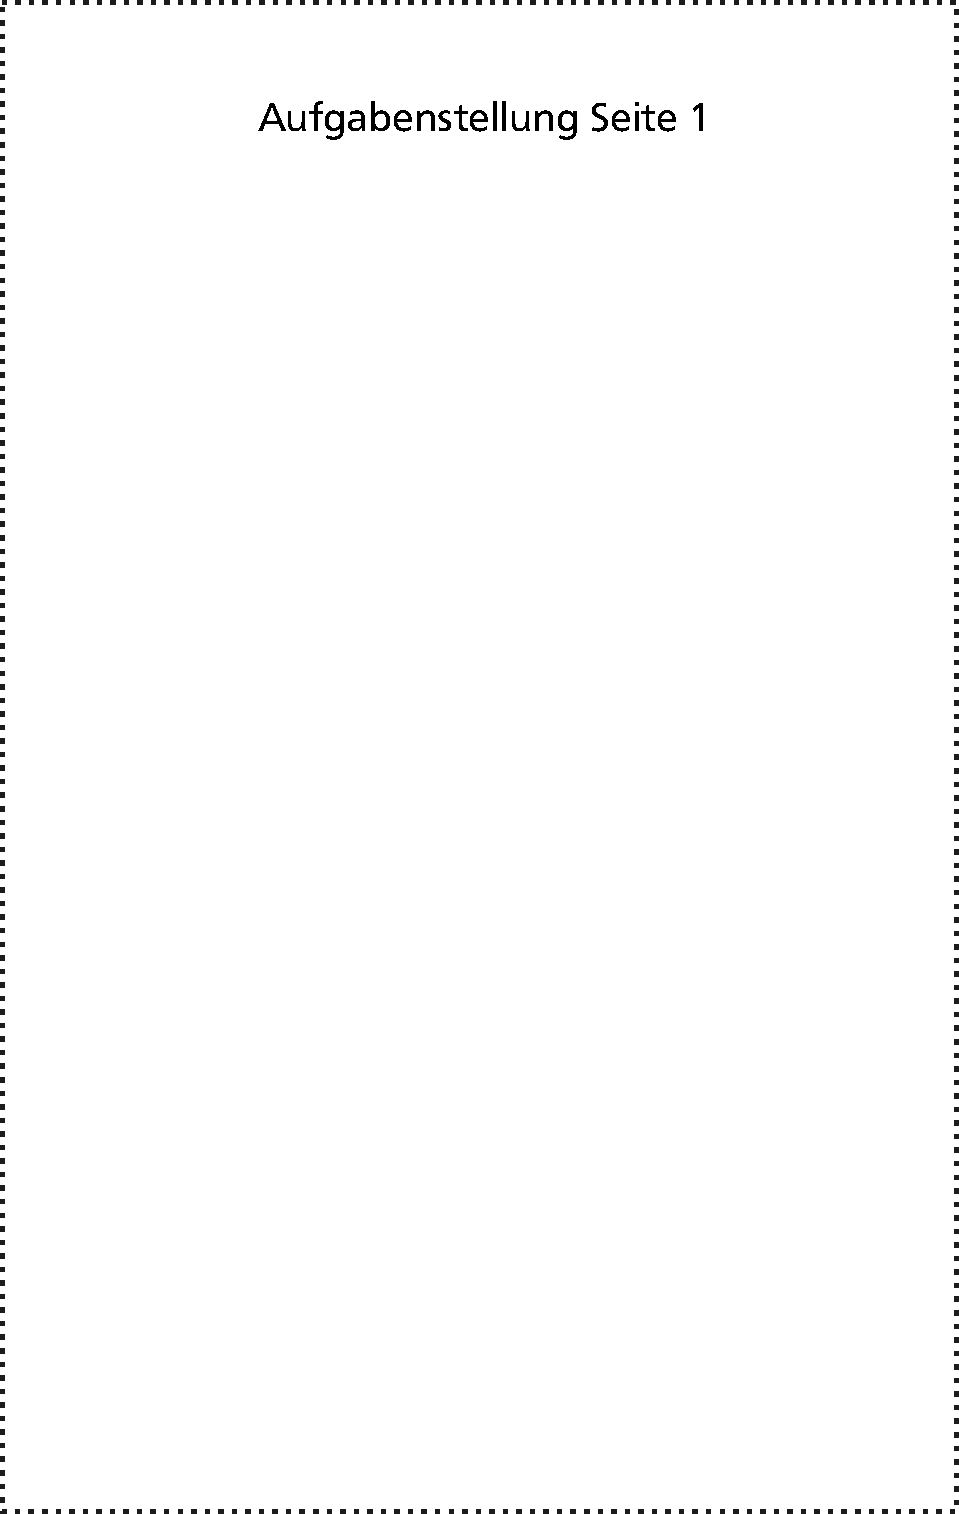
\includepdf[pages = 1, scale = 1.0, frame = true]{Aufgabenstellung/Aufgabenstellung_einseitig.pdf}

%\includepdf[pages = 2, scale = 1.0, frame = true]{Aufgabenstellung/Aufgabenstellung_zweiseitig.pdf}
%falls Aufgabenstellung 2 Seiten umfasst

%%%%% Leere Seite einfügen für doppelseitigen Druck (nicht nötig, wenn Aufgabenstellung 2 Seiten umfasst oder Abgabe nur digital%%%%
%\newpage 
%\thispagestyle{empty}
%\quad 
%\newpage
%%%%%%%%%%%%%%%%%%%%%%%%%%%%%%%%%

\pagenumbering{roman}

%\begin{affidavit*}[ngerman]{Erklärung zur Abschlussarbeit gemäß §\,22 Abs.~7 und APB der TU Darmstadt}

\ifdocenglish
    \begin{affidavit*}[ngerman]{Thesis Statement pursuant to §\,22 paragraph 7 of APB TU Darmstadt}
    %\textbf{Thesis Statement pursuant to §\,22 paragraph 7 of APB TU Darmstadt}
    
    I herewith formally declare that I, .........., have written the submitted thesis independently pursuant to §\,22 paragraph 7 of APB TU Darmstadt without any outside support and using only the quoted literature and other sources. I did not use any outside support except for the quoted literature and other sources mentioned in the paper. I have clearly marked and separately listed in the text the literature used literally or in terms of content and all other sources I used for the preparation of this academic work. This also applies to sources or aids from the Internet. This thesis has not been handed in or published before in the same or similar form. I am aware, that in case of an attempt at deception based on plagiarism (§\,38 Abs.~2 APB), the thesis would be graded with 5,0 and counted as one failed examination attempt. The thesis may only be repeated once.
    \\\\\\\\
    Date: \today\\
      \hspace*{\fill}\begin{tabular}{@{}l@{}}\hline
  \makebox[8cm]{Forename Surname}
  \end{tabular}
  \end{affidavit*}
\else
    \begin{affidavit*}[ngerman]{Erklärung zur Abschlussarbeit gemäß §\,22 Abs.~7 und APB der TU Darmstadt}
    Hiermit erkläre ich, ........., dass ich die vorliegende Arbeit gemäß §\,22 Abs.~ 7 APB TU Darmstadt selbstständig, ohne Hilfe Dritter und nur mit den angegebenen Quellen und Hilfsmitteln angefertigt habe. Ich habe mit Ausnahme der zitierten Literatur und anderer in der Arbeit genannter Quellen keine fremden Hilfsmittel benutzt. Die von mir bei der Anfertigung dieser wissenschaftlichen Arbeit wörtlich oder inhaltlich benutzte Literatur und alle anderen Quellen habe ich im Text deutlich gekennzeichnet und gesondert aufgeführt. Dies gilt auch für Quellen oder Hilfsmittel aus dem Internet. Diese Arbeit hat in gleicher oder ähnlicher Form noch keiner Prüfungsbehörde vorgelegen. Mir ist bekannt, dass im Falle eines Plagiats (§\,38 Abs.~2 APB) ein Täuschungsversuch vorliegt, der dazu führt, dass die Arbeit mit 5,0 bewertet und damit ein Prüfungsversuch verbraucht wird. Abschlussarbeiten dürfen nur einmal wiederholt werden.  
    \\\\\\\\
    Datum: \today\\
        \hspace*{\fill}\begin{tabular}{@{}l@{}}\hline
    \makebox[8cm]{Vorname Nachname}
    \end{tabular}
    \end{affidavit*}
\fi
	
	%Die folgenden Einträge beliebig erweitern oder löschen
	%\vspace{5mm}
	%\hspace*{\fill}\begin{tabular}{@{}l@{}}\hline
	%	\makebox[8cm]{\NameB}
	%\end{tabular}
	
	%\vspace{5mm}
	%\hspace*{\fill}\begin{tabular}{@{}l@{}}\hline
	%	\makebox[8cm]{\NameC}
	%\end{tabular}

%\end{affidavit*}

\cleardoublepage % Leere Seite einfügen für doppelseitigen Druck

\section*{Kurzfassung}
Eine halbe Seite Kurzfassung auf Deutsch

Schlüsselbegriffe: Digitaler Zwilling, Internet der Dinge, Virtuelle Produktentwicklung

\section*{Abstract}
Eine halbe Seite Kurzfassung auf Englisch

Keywords: Digital Twin, Internet of Things, Virtual product development

\cleardoublepage % Leere Seite einfügen für doppelseitigen Druck

\tableofcontents % Inhaltsverzeichnis
\cleardoublepage
\listoffigures % Abbildungsverzeichnis
\ifdocenglish
    \addcontentsline{toc}{chapter}{List of figures} % erzeugt einen Eintrag im Inhaltsverzeichnis
    \cleardoublepage
    \listoftables % Tabellenverzeichnis
    \addcontentsline{toc}{chapter}{List of tabels} % erzeugt einen Eintrag im Inhaltsverzeichnis
\else
    \addcontentsline{toc}{chapter}{Abbildungsverzeichnis} % erzeugt einen Eintrag im Inhaltsverzeichnis
    \cleardoublepage
    \listoftables % Tabellenverzeichnis
    \addcontentsline{toc}{chapter}{Tabellenverzeichnis} % erzeugt einen Eintrag im Inhaltsverzeichnis
\fi
\cleardoublepage
\ifdocenglish
  \chapter*{Abbreviations}
\else
  \chapter*{Abkürzungen}
\fi
\addcontentsline{toc}{chapter}{Abkürzungsverzeichnis} % erzeugt einen Eintrag im Inhaltsverzeichnis

%\section*{Operatoren und Funktionen}
%\begin{tabularx}{\textwidth}{@{}l@{\qquad}X@{\quad}p{18mm}}
%	\toprule
%	Symbol & Beschreibung & \\ \midrule
%	$*$ & Faltung\\
%	$\star$ & Kreuzkorrelation\\
%	$\delta(\cdot)$ & Dirac-Funktion\\
%	$\frac{\partial f}{\partial x}$ & partielles Differential\\
%	$\frac{\mathrm{d} f}{\mathrm{d} t}$ & totales Differential\\
%	$\Theta(\cdot)$ & Heaviside-/Sprung-Funktion\\
%\end{tabularx}


%\section*{Lateinische Symbole und Formelzeichen}
%\begin{longtable}{@{}l@{\qquad}p{0.72\columnwidth}@{\quad}p{18mm}}
%	\toprule
%	Symbol & Beschreibung & Einheit\\ \midrule
%	\endfirsthead
%	\toprule
%	Symbol & Beschreibung & Einheit\\ \midrule
%	\endhead
	
%	$A$ & Bauteilfl"ache in der $x$-$z$-Ebene & $\si{\square \milli \metre}$ \\
%	$a_\mathrm{f}$ & Parameter der Kaltflie{\ss}kurve & $\si{\newton \per \square \milli \metre}$\\
%	$b$ & Integrationskonstante & $\si{\newton}$\\
%	$b_\mathrm{f}$ & Parameter der Kaltflie{\ss}kurve & $\si{\newton \per \square \milli \metre}$\\
%	$E$ & Elastizit"atsmodul & $\si{\newton \per \square \milli \metre}$ \\
%	$F$ & aktuelle Reaktionskraft des Bauteils & $\si{\newton}$ \\
%	$F_m$ & Reaktionskraft des Bauteils zu Beginn der $m$-ten Entlastung & $\si{\newton}$ \\
%	$\bar{F}_m$ & Reaktionskraft des Bauteils nach der $m$-ten Entlastung & $\si{\newton}$\\
%	$F_n$ & Reaktionskraft des Bauteils im $n$-ten Abtastschritt & $\si{\newton}$ \\
%	$h$ & Bauteilh"ohe & $\si{\milli \metre}$\\
%	$I_y$ & Fl"achentr"agheitsmoment um die $y$-Achse & $\si{\milli \metre \tothe{4}}$ \\
%	$k$ & Bauteilsteifigkeit & $\si{\newton \per \milli \metre}$ \\
%	$k_\mathrm{f}$ & Flie{\ss}spannung der Kaltflie{\ss}kurve & $\si{\newton \per \square \milli \metre}$\\
%	$l$ & Bauteill"ange & $\si{\milli \metre}$ \\
%	$l_\mathrm{eff}$ & effektive Bauteill"ange zwischen den Auflagern & $\si{\milli \metre}$ \\
%	$M_\mathrm{y}$ & Biegemoment um die $y$-Achse & $\si{\newton \milli \metre}$ \\
%	$t$ & Zeit & $\si{\second}$ \\
%	$U$ & Steuerspannung des Proportionalventils & $\si{\volt}$\\
%	$\dot{V}$ & Volumenstrom durch das Proportionalventil & $\si{\cubic \milli \metre}$ \\
%	$w$ & aktuelle Bauteildurchbiegung & $\si{\milli \metre}$ \\
%	$w_n$ & Bauteildurchbiegung im $n$-ten Abtastschritt & $\si{\milli \metre}$ \\
%	$w_m$ & Bauteildurchbiegung zu Beginn der $m$-ten Entlastung & $\si{\milli \metre}$ \\
%	$\dot{w}$ & aktuelle Biegegeschwindigkeit & $\si{\milli \metre \per \second}$ \\
%	$w_0$ & Anfangsbauteildurchbiegung & $\si{\milli \metre}$\\
%\end{longtable}


%\section*{Griechische Symbole und Formelzeichen}
%\begin{longtable}{@{}l@{\qquad}p{0.72\columnwidth}@{\quad}p{18mm}}
%	\toprule
%	Symbol & Beschreibung & Einheit\\ \midrule
%	\endfirsthead
%	\toprule
%	Symbol & Beschreibung & Einheit\\ \midrule
%	\endhead
%	$\epsilon$ & Rauschprozesses der Kraftmessung & $\si{\newton}$\\
%	$\varepsilon$ & mechanische Dehnung & \\
%	$\varepsilon_\mathrm{el}$ & elastische Dehnung & \\
%	$\varepsilon_\mathrm{pl}$ & plastische Dehnung & \\
%	$\eta$ & Verfestigungsexponent des Bauteils & \\ 
%	$\eta_\mathrm{f}$ & Verfestigungsexponent der Kaltflie{\ss}kurve &\\ 
%	$\lambda$ & Vergessensfaktor & \\
%	$\mu_\mathrm{R}$ & Reibungskoeffizient & \\
%	$\nu$ & Rauschprozess der Wegmessung & \\
%	$\rho_0$ & Kr"ummungsradius des Balkens & \\
%	$\sigma$ & mechanische Spannung & $\si{\newton \per \milli \metre}$\\
%	$\sigma^2_\epsilon$ & Varianz der Kraftmessung & $\si{\square \newton}$ \\
%	$\sigma^2_\nu$ & Varianz der Wegmessung & $\si{\square \milli \metre}$ \\
%	$\sigma^2_\mathrm{F}$ & Varianz der Zufallsvariable $F$ & $\si{\square \newton}$ \\
%	$\varphi$ & Umformgrad & \\
%\end{longtable}


%\section*{Abk"urzungen}
\begin{longtable}{@{}l@{\qquad}p{0.72\columnwidth}@{\quad}p{18mm}}
	\toprule  
    \ifdocenglish
	   Abbreviation & full name & \\ 
    \else 
          Kürzel & vollständige  & \\ 
    \fi
    \midrule
	\endfirsthead
    ADP &  Advanced Design Project &\\
    ARP &  Advanced Research Project &\\
	CA &   Computer Aided, \textit{dt.:} rechnergestützt & \\
	CAD &  Computer Aided Design, \textit{dt.:} rechnergestütztes Konstruieren & \\
	CAE &  Computer Aided Engineering &\\

	DMU &  Digital Mock-Up & \\

    IoT &  Internet of Things, \textit{dt.:} Internet der Dinge & \\

	MBSE &  Model-Based Systems Engineering  & \\
	
	PDM & Produktdatenmanagement & \\
	PLM &  Product Lifecycle Management \textit{dt.:} Produktlebenszyklusmanagement & \\
	PLCM & Fachgebiet Product Life Cycle Management & \\
	
	SDM &  Simulationsdatenmanagement \\
	SE &  Systems Engineering  & \\
	STEP &  Standard for Exchange of Product Model Data  & \\	
	SysML &  Systems Modeling Language & \\	

	UML &   Unified Modeling Language & \\

\end{longtable}

 % Symbole und Abkürzungen

\mbox{}

%%%%%%%%%%%%%%%%%%%%%%%%%%%%%%
%Hier beginnt das eigentliche Dokument!!!
%%%%%%%%%%%%%%%%%%%%%%%%%%%%%

%\onehalfspacing %erhöht den Zeilenabstand auf 1.5-fach
\cleardoublepage
\chapter{Einleitung}
\label{ch:Einleitung}
\setcounter{page}{1}
\pagenumbering{arabic}

Dies ist die Vorlage zum Zitieren nach den Richtlinien der IEEE Editorial Style Manual (IEEE-Style).

Das Literaturverzeichnis ist nach Chronologie geordnet.  Die Referenz, die im Text zuerst genannt wird, steht auch im Literaturverzeichnis zuerst. 


Damit Kompilierung funktioniert, muss 
\begin{enumerate}
    \item unter Menu als Compiler \glqq LulaTeX\grqq~und als Main document \glqq PLCM-Thesis.tex\grqq~ausgewählt werden (siehe Abb.~\ref{fig:Kompilierung}) sowie 
    \item in einer tex-Datei neuer Text eingefügt werden.
\end{enumerate}

\begin{figure}[H]
	\begin{center}
		\centering
        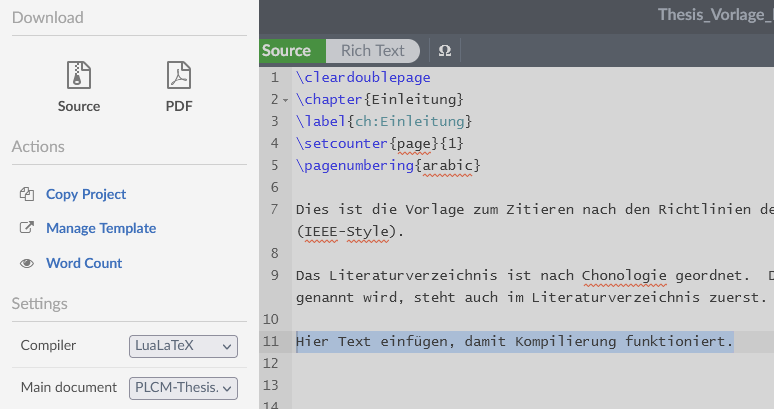
\includegraphics[width=\textwidth]{Bilder/Kapt1/Kompilierung.png}
		\caption{\centering Kompilierungseinstellungen}
		\label{fig:Kompilierung}
	\end{center}
\end{figure}

\section{Motivation}
\label{sec:Motivation}


\section{Zielsetzung}
\label{sec:Zielsetzung}

\section{Aufbau der Arbeit}
\label{sec:Aufbau}

\cleardoublepage
\chapter{Stand der Technik und der Forschung}
\label{ch:Stand_der_Technik}

\section{Art der Abschlussarbeit}
Je nach Art der Abschlussarbeit muss die Vorlage eigenständig angepasst werden. 
Der Typ der Arbeit wird auf der Titelseite in der \textit{Documentclass} in der Datei \textit{PLCM-Thesis.tex} angepasst.  

\section{Aufgabenstellung}
\begin{sloppypar}
\begin{itemize}
    \item Bei externen Arbeiten muss vorher ein Antrag zur Genehmigung der externen Arbeit gestellt werden. Hier muss der Titel der Arbeit schon feststehen und die Aufgabenstellung darf nach den Vorgaben des PLCM keinen Sperrvermerk enthalten.

    Weitere Informationen beim MechCenter unter \href{https://www.maschinenbau.tu-darmstadt.de/studieren/studierende/studium_bachelor/abschlussarbeiten_bachelor/index.de.jsp}{Bachelorarbeiten}  bzw. \href{https://www.maschinenbau.tu-darmstadt.de/studieren/studierende/studium_master/abschlussarbeit/index.de.jsp}{Masterarbeiten} \\
    oder auf dem Merkblatt Abschlussarbeiten der TU Darmstadt:
    \href{https://www.tu-darmstadt.de/media/dezernat_ii/referat_iig/fuer_pruefende/merkblaetter/info_externe_abschlussarbeiten.pdf}{Merkblatt}

    \item Die Aufgabenstellung wird vom Betreuer erstellt und muss vor Ausgabe an den Studenten von Herrn Prof. Schleich genehmigt werden. 

    \item Die Aufgabenstellung muss bei einer Bachelor-/Masterthesis auf eine Seite passen. Bei einer Aufgabenstellung eines Advanced Design Projects (ADP) bzw. Advanced Research Projects (ARP) dürfen es auch zwei Seiten sein. Auf der Aufgabenstellung steht auch der englische Titel der Arbeit. 

    \item Die Aufgabenstellung wird mit dem Studenten besprochen und ggf. angepasst. 

    \item Alles, was in der Aufgabenstellung steht, muss auch gemacht werden. Je allgemeiner formuliert, desto mehr Handlungsspielraum besteht während der Bearbeitungszeit und bei der Bewertung der Ausarbeitung.


    \item Nach Abgabe der Aufgabenstellung durch den Studenten im MechCenter, sollte der Student überprüfen, ob der Titel in \href{https://www.tucan.tu-darmstadt.de}{TUCaN} richtig eingetragen ist. 

\end{itemize}

Kontakt \href{https://www.maschinenbau.tu-darmstadt.de/studieren/mechcenter_studienbuero/pruefungsangelegenheiten/index.de.jsp}{MechCenter} -- Prüfungsangelegenheiten:\\ pruefungsmanagement@mechcenter.tu-darmstadt.de 

\end{sloppypar}


\section{Austausch von Dateien}
\begin{itemize}

    \item Zum Austausch von Dateien legt der Betreuer einen Ordner in der \href{https://next.hessenbox.de/shibboleth-ds/index.html?entityID=https%3A%2F%2Fnext.hessenbox.de%2Fshibboleth&return=https%3A%2F%2Fnext.hessenbox.de%2FShibboleth.sso%2FLogin%3FSAMLDS%3D1%26target%3Dss%253Amem%253Ab869f007763b2d33bdeb1bddb90fe9367a6913159761f53f4ed9cdc768118a2e}{next.Hessenbox} an. Dieser Ordner hat die einheitliche Ordnerstruktur mit den Unterordnern:
    \begin{itemize}
    \item 00\_Abgabe
    \item 01\_Orga
    \item 02\_Treffen
    \item 03\_Inhalt
    \item 04\_Ausarbeitung
    \item 05\_Kolloquium
    \end{itemize}
    
    
    Abgabe, Ausarbeitung, Literatur, Citavi, Präsentation, Organisatorisches, Analyse, Versuche, Veröffentlichung. 
    \item Dateinamen immer \textbf{ohne} Leerschritte schreiben. Bei Dateinamen dürfen Buchstaben a-z und A-Z, Ziffern 0-9, Minus/Bindestriche - und Unterstriche verwendet werden.  
    \item Sinnvolle Benennung für Dateien verwenden. 
    \item Zwischenversionen speichern
    \item Speicherkopien des Hessenboxordners erstellen. Dafür empfiehlt sich eine Backup Software, wie bspw. Veeam Agent.
\end{itemize}

\section{Organisatorisches zwischen Betreuer und Student}
\begin{itemize}
    \item geplante Urlaube/Abwesenheiten mitteilen
    \item Regeltermine vereinbaren
    \item klären, wie viele Seiten die Ausarbeitung etwa haben soll
    \item klären, wie viele Wochen vor finaler Endabgabe die fertige Version an den Betreuer geschickt werden soll
\end{itemize}

\section{Corporate Design}

\begin{sloppypar}
Infos zum Corporate Design der TU Darmstadt sind unter \url{https://www.intern.tu-darmstadt.de/arbeitsmittel/corporate_design_vorlagen/index.de.jsp} zu finden.\\
Dazu zählen Vorlagen, Schriften und Farben. 
\end{sloppypar}

\subsection{Vorlagen}

\begin{itemize}
    \item Die schriftliche Ausarbeitung kann in Word oder in LaTeX verfasst werden. 

    \item Über \href{https://sharelatex.tu-darmstadt.de/}{ShareLaTeX TU-Darmstadt}  können Vorlagen für Abschlussarbeiten angepasst und verwendet werden. Dabei muss die Farbe der Titelseite und der Balken auf jeder Seite auf das PLCM-Blau angepasst werden, siehe \ref{subsec:farbe}. 

    \item Weiter Infos zu \href{https://www.hrz.tu-darmstadt.de/services/it_services/sharelatex_hrz/index.de.jsp}{ShareLaTeX}

    \item Die LaTeX- bzw. Word-Vorlage sowie die PowerPoint-Vorlage werden über die Hessenbox zur Verfügung gestellt. 
\end{itemize}

\subsection{Schriften}
\begin{itemize}
    \item Charter für Fließtexte
    \item Frontpage für Überschriften
    \item Bei Präsentationen müssen andere Schriften verwendet werden!
\end{itemize}

\subsection{Farbe}
\label{subsec:farbe}
Das PLCM-Blau ist die Farbe 1b in der Farbpalette: RGB-Code ist 0 90 169 und Hex-Code 005AA9.

\section{Hinweise zur Gestaltung wissenschaftlicher Arbeiten}

\subsection{Aufbau, Inhalt und wissenschaftlichen Schreiben}


\begin{enumerate}
    \item Die Gliederung wird mit dem Betreuer abgesprochen.
    \item Der Kern der Arbeit muss nach der Einleitung verstanden sein. 
    \item Das Kapitel zum Stand der Technik und Forschung sollte den Kern der Arbeit treffen und nicht zu breit angelegt sein. Hier sollten Begriffe und Themen eingeführt werden, um den Rest der Ausarbeitung zu verstehen. 
    \item Das Kapitel \glqq Konzept\grqq~sollte ausführlich sein, da das Konzept der Kern der Arbeit ist. 
    \item Es sollten vorwiegend wissenschaftliche Publikationen als Referenzen verwendet werden. Zudem sollten unterschiedliche Quellen verwendet werden. Bei längeren Quellen ist die Seitenzahl im Verweis mitanzugeben.
    \item Die Ausarbeiten soll im Präsens Passiv verfasst sein. Zum Beispiel: \glqq Es wird eine Konzept erarbeitet.\grqq~  Ausnahme ist hierbei die Zusammenfassung (Präteritum Passiv): \glqq Es wurde eine Konzept erarbeitet.\grqq~
    \item  Keine \grqq Man \grqq~ -Sätze, keine \glqq Könnte\grqq -Sätze (Konjunktive vermeiden), Keine \glqq Ich/Wir\grqq  -Sätze, keine Bandwurmsätze
    \item Richtwerte für Umfang
    \begin{enumerate}
        \item B\;Sc.: 60 Seiten 
        \item B\;Sc.: 80 Seiten
        \item ADP/ARP: 15-20 Seiten pro Person
    \end{enumerate}
    \item Einheitliche Formatierung sowie einheitliches Design der Abbildungen \& Tabellen
    \item Unterkapitel maximal bis zur dritten Ebene (z.B.: 3.3.2). Bei Verwendung von Unterkapiteln mindestens zwei Unterkapitel verwenden
    \item Keine Umgangsprache verwenden und Regeln der Rechtschreibung beachten.
    \item Keine Umgangssprache verwenden und Regeln der Rechtschreibung beachten
    \item Vorsicht bei Wertung (exkl. Fazit)
\end{enumerate}

\subsection{Rechtschreibung und Typografie}

\begin{enumerate}

    \item Es sollten für den gleichen Sachverhalt der gleiche Begriff verwendet werden.
    \item Die Verwendung von Abkürzungen muss eingeführt werden: 
    Alle verwendeten Abkürzungen, die nicht im Duden stehen, müssen im Abkürzungsverzeichnis aufgeführt sein. Es wird in zwei Arten von Abkürzungen unterschieden:
    
    \begin{enumerate}
        \item Abkürzung ist in der gleichen Sprache wie die entsprechende Bezeichnung: Finite-Elemente-Methode (FEM), Model-Based Systems Engineering (MBSE)
        \item Abkürzung ist in einer anderen Sprache als die entsprechende Bezeichnung: Internet der Dinge (IoT, \textit{engl.: Internet of Things})
    \end{enumerate}

    
    \item Am Satzanfang \glqq zum Beispiel\grqq~ und \glqq beispielsweise\grqq~ ausschreiben und nicht die Abkürzungen z.\,B. bzw. bspw. verwenden.
    \item Lieber das Wort \glqq Thesis\grqq~statt \glqq Arbeit\grqq~verwenden. Zum Beispiel: In dieser Masterthesis wird der Schwerpunkt auf [...] gelegt. 
    \item Es sollen bedingte Trennstriche verwendet werden, um den Blocksatz möglichst gut auszunutzen. Die Abstände zwischen den einzelnen Wörtern soll nicht zu groß werden, damit der Text gut lesbar bleibt. Mit einem bedingten Trennstrich kann festgelegt werden, wo ein Wort getrennt werden soll, falls es getrennt werden muss. An dieser Stelle z.\,B.: Produktlebens"-phasen.
    \item Bei Abkürzungen, Seitenangaben, Paragraphen und Einheiten sollen schmale Leerzeichen verwendet werden:\\
     B.\,Sc., M.\,Sc., z.\,B., e.\,V., d.\,h., S.\,234\,f., Abs.\,1, §\,123 BGB, 20\,€, 2-5\,\% 
    \item Geschützte Leerzeichen ermöglichen es, zwischen Wörtern, Zahlen und Zeichen einen Zeilenwechsel zu verhindern. Zum Beispiel bei Eigennamen: Industrie~4.0
    \item Vor und nach einem Schrägstrich gibt es keine Leerschritte. Zum Beispiel: Urlaube/Abwesenheiten.
    \item Normalerweise werden Komposita im Deutschen in einem Wort geschrieben. Es gibt aber Ausnahmen, in denen Komposita durchgekoppelt, also mit Bindestrichen verbunden werden: 
    \begin{enumerate}
        \item bei Komposita aus Zahlen, Wörtern und Sonderzeichen: Industrie-4.0-Vision
        \item bei Komposita mit Bestimmungswörtern (\textit{Produkt} und \textit{Service}), die sonst durch Leerzeichen getrennt werden: Produkt-Service-Systeme
    \end{enumerate}
    
\end{enumerate}

\subsection{Literaturempfehlung}
\begin{itemize}
    \item \citetitle{karmasin2013gestaltung} (\citeyear{karmasin2013gestaltung}) \textcite{karmasin2013gestaltung}.
    \item \citetitle{TheisenWissenschaftlichesArbeiten2021} (\citeyear{TheisenWissenschaftlichesArbeiten2021}) \textcite{TheisenWissenschaftlichesArbeiten2021}.
\end{itemize}

\section{Suchmaschinen für Literatur}
\label{sec:suchmasch}
\begin{sloppypar}

\begin{itemize}
    \item \href{http://scholar.google.de}{Google Scholar}
    \item \href{http://dakapo.ulb.tu-darmstadt.de/servlet/Top/searchadvanced}{ULB Darmstadt}
    \item \href{http://www.portal.hebis.de/servlet/Top/searchadvanced}{HeBIS} (für Fernleihe/über Betreuer)
    \item \href{https://link.springer.com/}{Springer Link}
    \item \href{https://www.ulb.tu-darmstadt.de/finden_nutzen/recherchieren/normen_richtlinien.de.jsp}{Nautos} (ehem. Perinorm) für DIN-Normen und VDI-Richtlinien
    \item \href{http://rzblx1.uni-regensburg.de/ezeit/}{Elektronische Zeitschriften}
    \item \href{http://www.sciencedirect.com/science/journals}{ScienceDirect}
    \item \href{https://www.semanticscholar.org/}{Semantic Scholar} Semantic Schlar 
    \item \href{https://www.webofscience.com/wos/woscc/basic-search}{Web of Science}
    \item \href{https://www.connectedpapers.com/}{Connected Papers}
\end{itemize}


\end{sloppypar}

\section{Zitation}
\label{sec:zitation}
\begin{itemize}
    \item Jede fremde Ansicht und jede Ansicht des Verfassers, die in einer anderen als der vorliegenden Arbeit schon einmal geäußert worden ist, muss zitiert werden. Die Herkunft aller Gedanken, Ergebnisse und Zitate, die aus anderen Werken übernommen wurden, müssen eindeutig belegt und im Text kenntlich gemacht werden. Die Nachweise können sich auf ein Wort, einen Satz, einen Absatz oder einen ganzen Abschnitt beziehen.
    \item Es soll vermieden werden, dass ein ganzer Absatz sich auf eine Referenz bezieht. Lediglich sollen ein bis zwei Sätze aus einer Referenz stammen. 

    \item \textbf{Indirekte Zitate}: Wird ein Autor sinngemäß wiedergegeben, so ist dies nach der Textpassage kenntlich zu machen. Drei Möglichkeiten gibt es:

    \begin{enumerate}
        \item Die Erreichung der virtuellen Produktentstehung kann in mehrere Ebenen eingeteilt werden \cite{anderl_simulations}.
        \item \textcite{anderl_simulations} teilt die Erreichung der virtuellen Produktentstehung in mehrere Ebenen. 
        \item In \citeyear{anderl_simulations} teilt \cite{anderl_simulations} die Erreichung der virtuellen Produktentstehung in mehrere Ebenen.  
    \end{enumerate}
    \item \textbf{Direkte Zitate}: Wörtliche Zitate sind zwischen Anführungszeichen zu setzen und die genaue Seite muss angegeben werden. Diese Zitierweise sollte vermieden werden.
\end{itemize}


\subsection{Literaturverwaltungsprogramme}
\begin{sloppypar}
\textbf{Zotero}
    \begin{itemize}
        \item Download der kostenfreien Software: \href{https://www.zotero.org/}{Zotero}
    \end{itemize}
    
\textbf{Citavi}
    \begin{itemize}
        \item Download der \href{https://www.ulb.tu-darmstadt.de/service/literaturverwaltung_start/citavi_ulb/citavi_ulb.de.jsp}{Software Citavi Free}
        
        \item \href{https://citaviweb.citavi.com/p/campus?signin=381c6aa567651c63bf9c923be02b4568&accountKey=r52j8qr0an1djhf7njobe6ry4svyc8sapuuboul020lh8xt3#usertype}{Lizenzdaten (kostenlos) anfordern und ggf. an ULB Tutorials/Schulungen teilnehmen}
    \end{itemize}
\end{sloppypar}

\clearpage

\subsection{Zitieren in LaTeX}
\label{subsec:ZitLaTeX}

\textbf{Zitieren}
\begin{itemize}
    \item ohne Seitenangabe \cite{anderl_simulations}
    \item mit Seitenangabe \cite[3-12]{anderl_simulations}
    \item Zitieren von mehreren Referenzen \cite{anderl_simulations, DissHaag}
\end{itemize}

\textbf{Zitieren in Abb. oder in den Text eingebaut:}
\begin{itemize}
    \item Nach \textcite{anderl_virtuelle_2020} ist der Produktentstehungsprozess Bestandteil des Produktlebenszyklus.
\end{itemize}

\textbf{Unterscheidung nach Literaturtyp}

Die Darstellung der Referenzen erfolgt im Literaturverzeichnis abhängig vom Literaturtyp.
Unterschieden wird dafür in der .bib-Datei in folgende Literaturtypen:

\begin{itemize}
    \item \textbf{book} für Bücher \cite{anderl_simulations}
    \item \textbf{incollection} für Kapitel oder Paper in einem Sammelband \cite{anderl_virtuelle_2020} 
    \item \textbf{article} für Paper \cite{shapingDT}  
    \item \textbf{thesis} für Dissertationen \cite{DissHaag}
    \item \textbf{online} für Onlinequellen \cite{PLCM}
    \item \textbf{misc} für Sonstiges, zum Beispiel VDI-Richtlinen \cite{VDI2206} und \cite{INCOSE2020} 
\end{itemize}


\subsection{UML-Diagramme}
Empfehlungen:
\begin{itemize}
    \item Lucidchart (Education Version)
    \item StarUML 
\end{itemize}

Kostenpflichtige Programme:
\begin{itemize}
    \item Microsoft Visio
    \item Cameo System Modeller\textsuperscript{\texttrademark}
    \item Visual Paradigm (Das PLCM hat eine Lizenz, bei Interesse den Betreuer fragen)
\end{itemize}



\section{Aussarbeitung}
\label{sec:Abschnitt}

\subsection{Anforderungen an Ausarbeitung}
\begin{itemize}
    \item Umfang (Richtwerte):
    \begin{itemize}
        \item B.\,Sc.: 60 Seiten
        \item B.\,Sc.: 80 Seiten
        \item ADP/ARP 15-20 Seiten pro Person
    \end{itemize}
    \item Gliederung nach Absprache
    \item Präsenz verwenden
    \item Einhaeitliche Formatierung
    \item Keine "Man"-Sätze
    \item Keine "Könnte"-Sätze (Konjungtive verwenden)
    \item Keine "Ich/Wir"-Sätze
    \item Keine Bandwurmsätze
    \item Vorsicht bei Wertung (exkl. Fazit)
    \item Rechtschreibung (Sprache beachten)
    \item Keine Umgangssprache
    \item Einheitliche Benennung
    \item Eigenen Grafiken als Vektorgrafik
    \item Beim Verwenden von Unterkapiteln mindestens zwei Unterkapitel vernwenden
    \item Unterschiedliche Quellen nutzen (Fachliteratur, Paper/Journals, Internet mit Abruf am...) \textbf{mit} Seitenzahl bei Verweisen!
    \item Unterkapitel maximal bis zur dritten 
\end{itemize}

\subsection{Latex-Hinweise}

\begin{itemize}
    \item \glqq Gänsefüßchen\grqq~werden so geschrieben.\footnote{Beispielfußnote}
    \item \textit{kursiv}, \textbf{fett}
    \item hochstellen km$^2$, tiefstellen H$_{2}$O
    \item Bindestrich und Wortergänzungsstrich -, bedingter Trennstrich "-, Gedankenstrich --
    \item schmales Leerzeichen z.\,B. für: e.\,V., d.\,h., B.\,Sc., M.\,Sc., S.\,234\,f., Abs.\,1, §\,123 BGB, 20\,€, 2-5\,\% und automatisch erzeugt bei SI-Einheiten \SI{225}{g/m^2}
    \item URL \url{www.pexels.com} 
\end{itemize}

Stichpunkten: 
\begin{itemize}
    \item Stichpunkt 1
    \item Stichpunkt 2
\end{itemize}

Stichpunkten und mehreren Ebenen:
\begin{itemize}
\item erste Ebene
\begin{itemize}
\item zweite Ebene
\begin{itemize}
\item dritte Ebene
\begin{itemize}
\item vierte Ebene
\end{itemize}
\end{itemize}
\end{itemize}
\end{itemize}


Aufzählungen mit Nummerierung: 
\begin{enumerate}
    \item Stichpunkt 1
    \item Stichpunkt 2
\end{enumerate}

Aufzählungen mit Nummerierung und mehreren Ebenen:
\begin{enumerate}
    \item Erste Ebene
    \begin{enumerate}
        \item Zweite Ebene
        \begin{enumerate}
            \item Dritte Ebene
            \begin{enumerate}
                \item Vierte Ebene
            \end{enumerate}
        \end{enumerate}
    \end{enumerate}
\end{enumerate}
%\begin{enumerate}
%\item erste Ebene
%\begin{enumerate}
%\item zweite Ebene
%\begin{enumerate}
%\item dritte Ebene
%\begin{enumerate}
%\item vierte Ebene
%\end{enumerate}
%\end{enumerate}
%\end{enumerate}
%\end{enumerate}

\subsection{Abbildungen}
\begin{sloppypar}
\begin{itemize}
    \item Für Abbildungen sollen Vektorgrafiken verwendet werden. Vektorgrafiken verpixeln nicht, wenn sie vergrößert werden. Mögliche Programme zum Erstellen von Vektorgrafiken als PDF-Datei sind \href{https://inkscape.org/de/}{Inkscape} und Power-Point.
    \item Icons sind zum Beispiel unter \href{https://www.flaticon.com/de/}{www.flaticon.com} und \href{https://thenounproject.com/}{www.thenounproject.com} zu finden. Icons werden zur Repräsentation von Themen genutzt. Besonders bei Kolloquiumpräsentationen des Kolloquium ist die Verwendung von Icons zu empfehlen. 
    \item Hier der Verweis auf Abb.~\ref{fig:Vektorgrafik} und Abb.~\ref{fig:EbeneVPEP}. Jede Abb. und jede Tab. muss mindestens einmal referenziert werden.
\end{itemize}

 \end{sloppypar}
 
\begin{figure}[H]
	\begin{center}
		\centering
		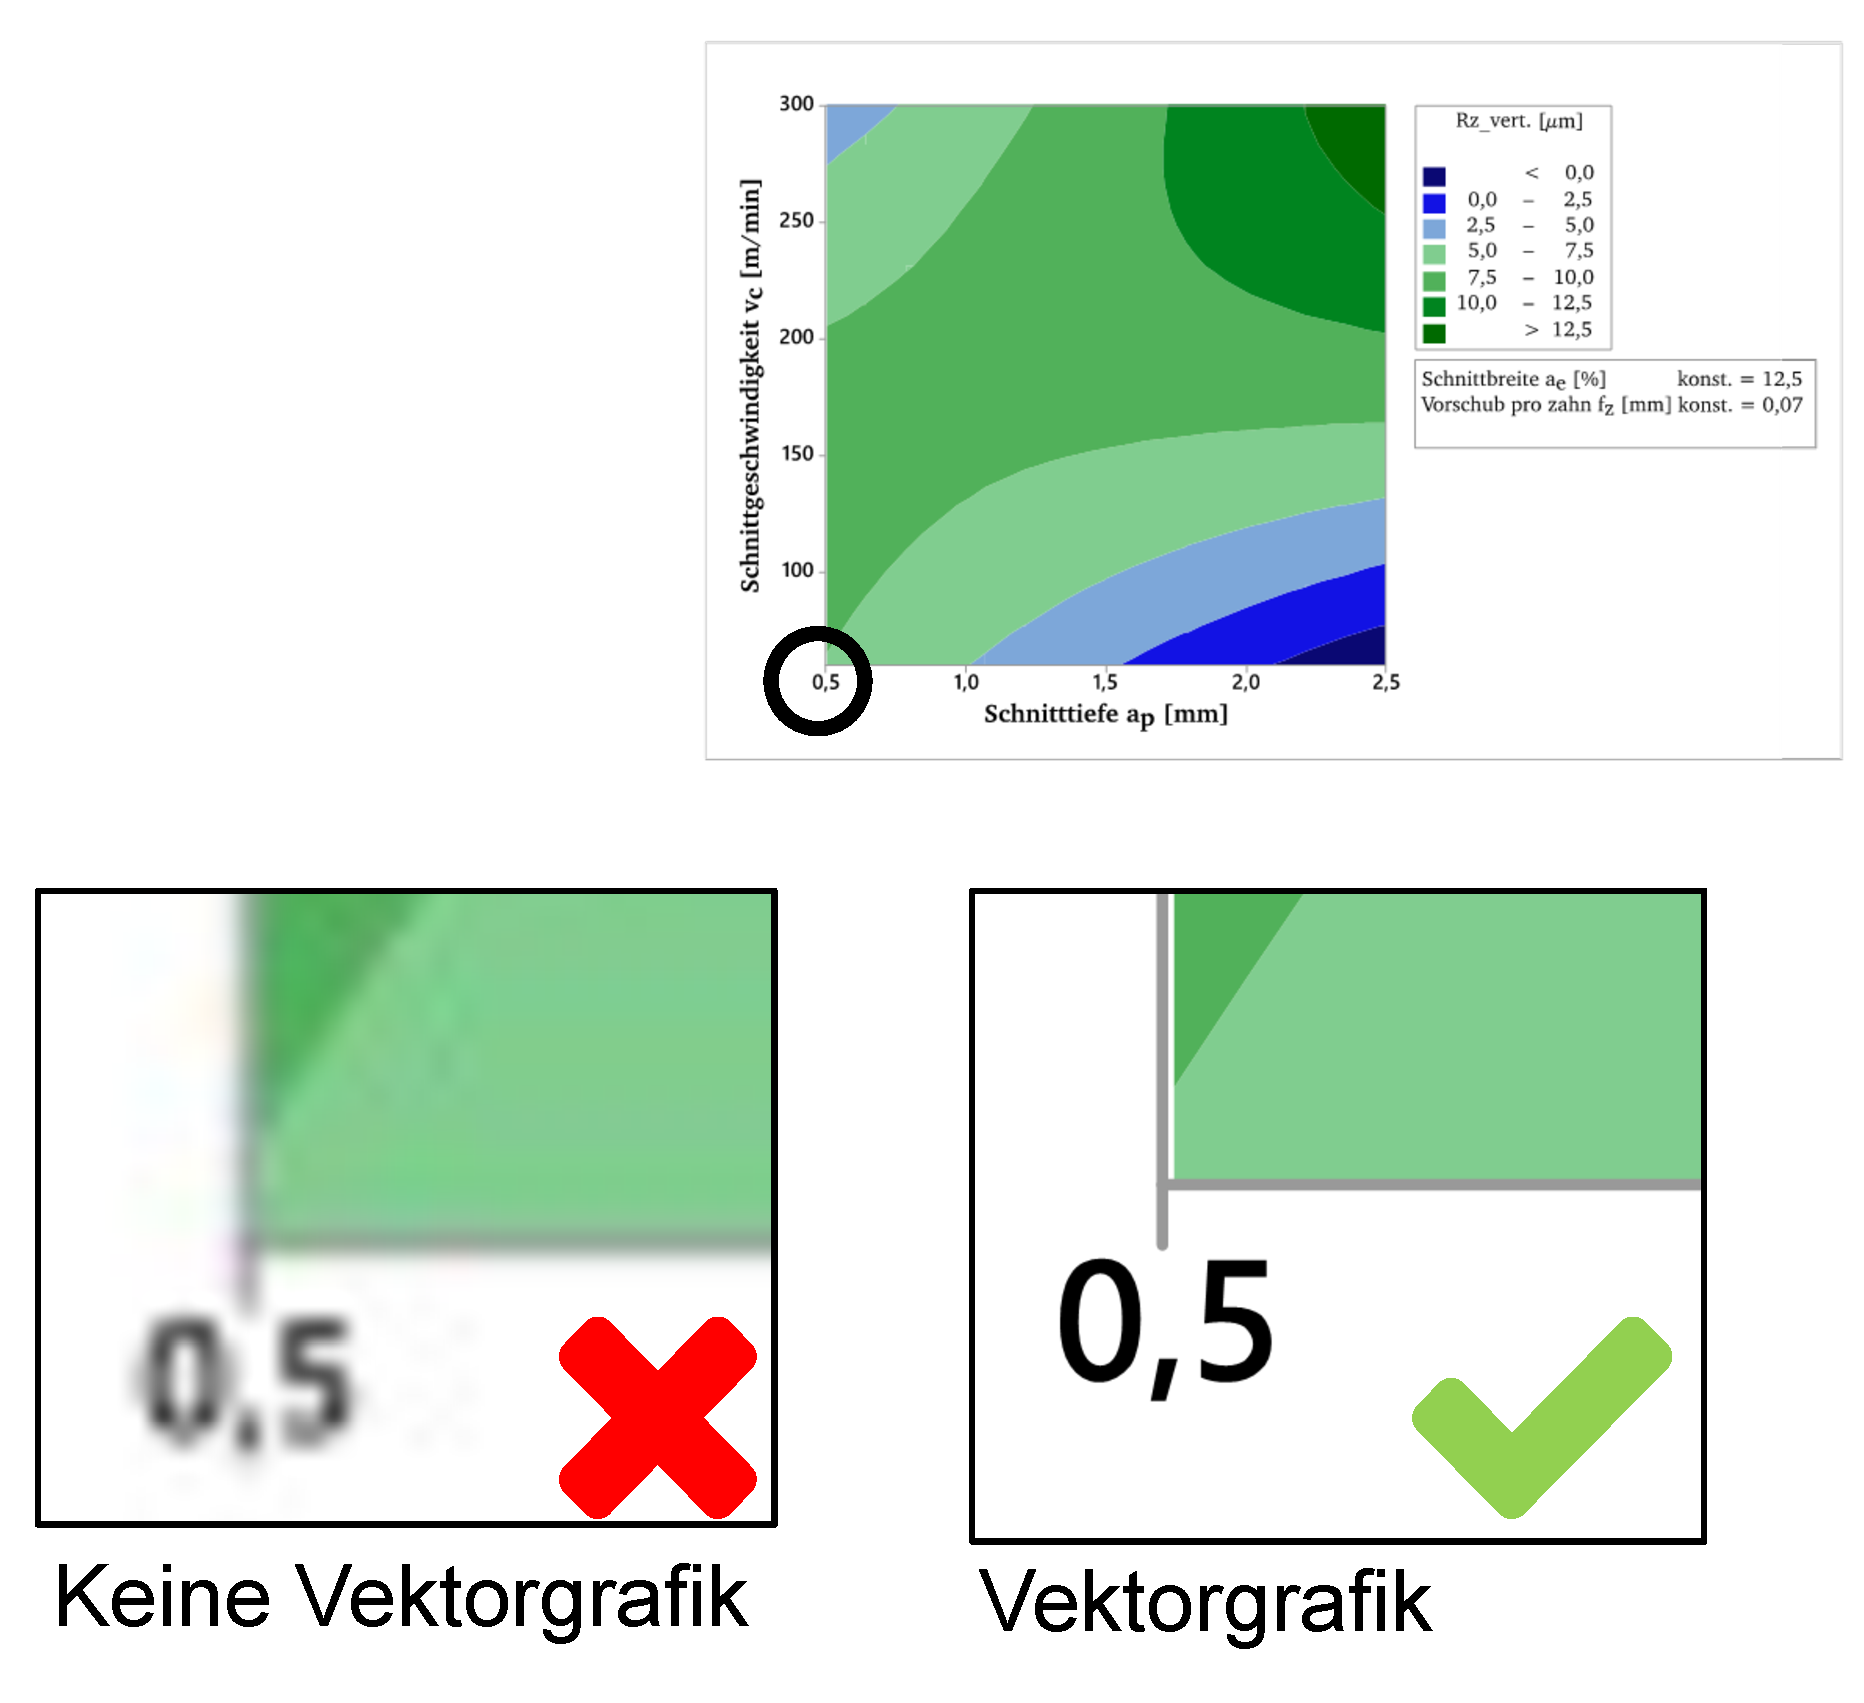
\includegraphics[width=0.5
		\textwidth]{Bilder/Kapt2/Vektorgrafik2.pdf}
		\caption{Vektorgrafik}
		\label{fig:Vektorgrafik}
	\end{center}
\end{figure}

\begin{figure}[H]
	\begin{center}
		\centering
		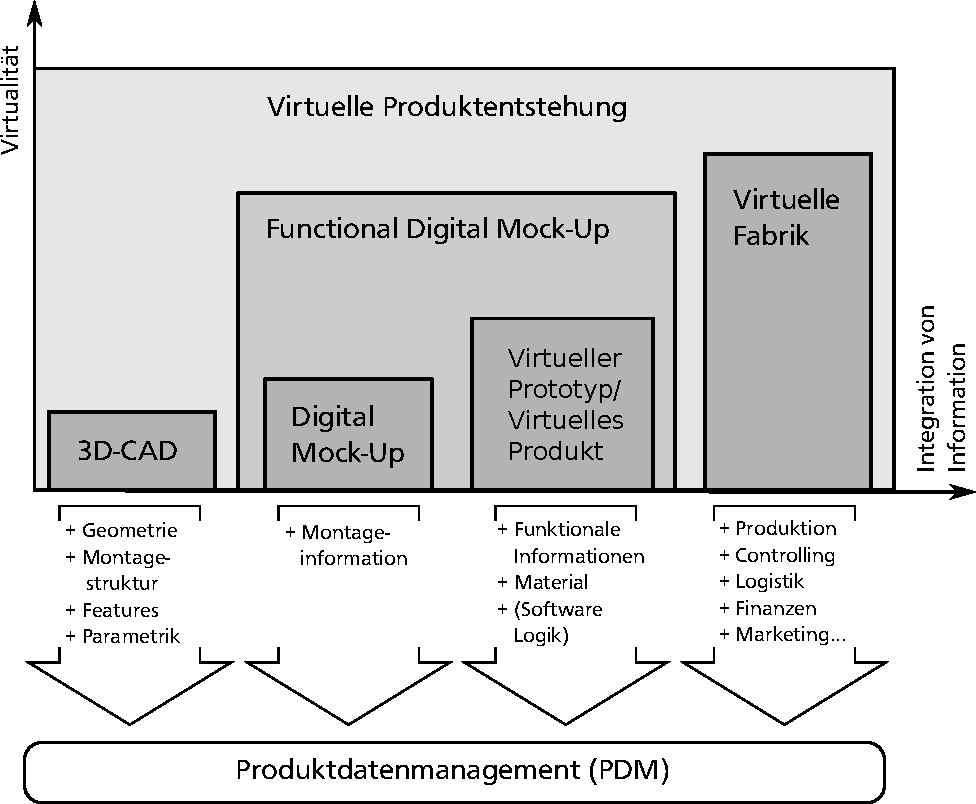
\includegraphics[width=0.6
		\textwidth]{Bilder/Kapt2/EbenenVPEP.pdf}
		\caption{Ebenen der virtuellen Produktentstehung nach \cite{anderl_simulations}}
		\label{fig:EbeneVPEP}
	\end{center}
\end{figure}

\subsection{Tabellen}
Hier der Verweis auf Tab.~\ref{tab:SIM}. Jede Abb. und jede Tab. muss mindestens einmal referenziert werden.
\FloatBarrier
\begin{table}[tbh]
	\centering
	\caption{\centering Simulationen unterschiedlicher Güte}
	\label{tab:SIM}
    \begin{tabular}{l|l|l|l}
	& SIM 1 & SIM 2 & SIM 3 \\
	\hline
	\hline
	Simulationsschritte & 100  & 300 & 3000 \\
	\hline
	Simulationszeit& \SI{50}{s} & \SI{30}{s} & \SI{10}{s} \\
	\hline
	\end{tabular}
\end{table}
\FloatBarrier

\section{Abgabe von Abschlussarbeiten}

\begin{sloppypar}
\begin{itemize}
    \item Die Abgabe der Thesis erfolgt entsprechend der Absprachen mit dem Betreuer einige Wochen vor der finalen und offiziellen Endabgabe.  
    
    \item Der Titel der schriftlichen Ausarbeitung muss identisch mit dem Titel sein, der in TUCaN bei der Anmeldung der Abschlussarbeit steht. 
    
    \item Die offizielle Endabgabe von Abschlussarbeiten erfolgt in elektronischer Form über TUbama (\url{https://tubama.ulb.tu-darmstadt.de/}). Weitere Infos unter: \url{https://www.tu-darmstadt.de/studieren/studierende_tu/studienorganisation_und_tucan/hilfe_und_faq/artikel_details_de_en_96256.de.jsp}
    Hierzu bitte die Vorgaben des MechCenters berücksichtigen.

    \item Weitere Informationen unter TUbama (\url{https://tubama.ulb.tu-darmstadt.de/})

\end{itemize}
\end{sloppypar}


\section{Lernziele von Abschlussarbeiten}

\begin{enumerate}
    \item Eine technisch-wissenschaftliche Fragestellung mit ingenieurwissenschaftlichen Methoden strukturiert zu lösen.
    \item Die Fragestellung kritisch zu bearbeiten und mögliche Lösungen einzuschätzen.
    \item Die Ergebnisse in schriftlicher und mündlicher Form mit wissenschaftlichen Anspruch zu präsentieren.
\end{enumerate}

\subsection*{Grundregeln des wissenschaftlichen Arbeitens}
\begin{itemize}
    \item Ergebnisse, Methoden und Verfahren sorgfältig und nachvollziehbar dokumentieren.
    \item Integre Argumentation bei wissenschaftlichen Auseinandersetzungen
    \begin{itemize}
        \item Klare Unterscheidung von Ergebnissen und deren Interpretation
    \end{itemize}
    \item Verantwortungsvolles Verhalten zwischen Student*in und Betreuer*in
    \item Zitation von Forschungsergebnissen, Publikationen und Ideen anderer Wissenschaftler*innen
    \item Verantwortungsvoller Umgang mit Daten und KI
    \begin{itemize}
        \item Siehe \href{https://www.maschinenbau.tu-darmstadt.de/media/maschinenbau/dokumente_2/studieren_1/thesis/2025-06-20_KI-Leitlinien_FB_MB.de.pdf}{Hilfsmittel} zum Umgang mit KI-Hilfsmitteln des Maschinenbaus.
        \item Siehe \href{https://www.hda.tu-darmstadt.de/hochschuldidaktik/infoseiten_hd/handreichung_ki_hd/handreichung_ki_verteilerseite.de.jsp}{Zentraler KI-Leitfaden} der TU Darmstadt
    \end{itemize}
\end{itemize}
\section{Weitere Links}
\begin{sloppypar}
\begin{itemize}
    \item Schreibgruppen vom SchreibCenter am Sprachenzentrum\\ (\url{https://www.owl.tu-darmstadt.de/angebote_vor_ort/schreibgruppen/schreibgruppen.de.jsp})
    \item Software vom HRZ\\
\url{https://www.hrz.tu-darmstadt.de/services/it_services/campus_software/index.de.jsp}
    \item GitLab Versionsverwaltung\\ \url{https://www.hrz.tu-darmstadt.de/services/it_services/gitlab/index.de.jsp}
    \item Normen und Regelwerke\\
\url{https://www.ulb.tu-darmstadt.de/finden_nutzen/recherchieren/normen_richtlinien.de.jsp}
    \item Kompilierungszeit verringern\\
Um die Kompilierungszeit der einzelnen Dateien zu verringern, kann die Ausarbeitung über das Package \textit{subfiles} organisiert werden. Eine Anleitung für die Umsetzung ist hier zu finden: \url{https://de.overleaf.com/learn/latex/Multi-file_LaTeX_projects}

\end{itemize}
\end{sloppypar}
\cleardoublepage

\chapter{Handlungsbedarf und Anforderungsdefinition}
\label{ch:Kapt3}

\section{Handlungsbedarf}
\label{sec:Handlungsgedarf}

\section{Zieldefinition}
\label{sec:Zieldefi}

\section{Anwendungsfälle}
\label{sec:Anwend}

\section{Anforderungen an die Methode}
\label{sec:AnfordMethode}


\cleardoublepage
\chapter{Konzept}
\label{ch:Konzept}

\section{Definitionen}
\label{sec:Def}

\section{Konzeptüberblick}
\label{sec:Konzeptueberblick}

\section{Methode}
\label{sec:Methode}

\cleardoublepage
\chapter{Anwendung der Methode}
\label{ch:AnwendMeth}

Dieses Kapitel wird auch häufig Implementierung genannt. 


\cleardoublepage
\chapter{Validierung der Methode}
\label{ch:Validerung}



\section{Fazit}
\label{sec:Fazit}


\cleardoublepage
\chapter{Ausblick und Zusammenfassung}
\label{ch:AusblickZsmfassung}

\section{Ausblick}
\label{sec:Ausblick }

\section{Zusammenfassung}
\label{sec:Zsmf}




\cleardoublepage
%\singlespacing %setzt den Zeilenabstand zurück auf einfach
\ifdocenglish
    \addcontentsline{toc}{chapter}{Bibliography}
    \printbibliography[title={Bibliography}]
\else
    \addcontentsline{toc}{chapter}{Literaturverzeichnis}
    \printbibliography[title={Literaturverzeichnis}]
\fi
%\onehalfspacing %erhöht den Zeilenabstand auf 1.5-fach
\cleardoublepage

% --- KI-Hilfsmittel-Verzeichnis ---
\chapter*{KI-Hilfsmittel-Verzeichnis}
\addcontentsline{toc}{chapter}{KI-Hilfsmittel-Verzeichnis}

KI-Hilfsmittel-Tabelle orientiert an der \href{https://www.ulb.tu-darmstadt.de/media/ulb/forschen_publizieren/ki/ki_empfehlung_kurz.de.pdf}{Vorlage} der TU Darmstadt ausfüllen.

\begin{longtable}{|p{0.175\textwidth}|p{0.175\textwidth}|p{0.175\textwidth}|p{0.175\textwidth}|p{0.175\textwidth}|}
\hline
\rowcolor[HTML]{C0C0C0} 
{\color[HTML]{DEDEDE} } \textbf{Einsatzform} \; (z.B. Formulierungsvorschläge, Textstrukturierung, Formulierung von Überschriften etc.) & {\color[HTML]{DEDEDE} } \textbf{Eigenleistung} (Intellektueller Beitrag; z.B. KI-Generat angepasst, Quellen ergänzt, Faktencheck etc.) & {\color[HTML]{DEDEDE} } \textbf{Betroffene
Teile der Arbeit} & {\color[HTML]{DEDEDE}}\textbf{KI-Hilfsmittel} \; (Name, ggf. Version und Anbieter) & {\color[HTML]{DEDEDE}} \textbf{Bemerkung} \;\; (Verweis auf einen Prompt- oder Gesprächsverlauf mit dem KI-Hilfsmittel)
 \\ \hline
\endfirsthead
\endhead
 &   &  &   &  \\ \hline


\end{longtable}   
%\cleardoublepage
%für den Anhang braucht man folgendes

\appendix
	\cleardoublepage
\
\ifdocenglish
    \chapter{Appendix}
\else
    \chapter{Anhang}
\fi
\label{app:Anhang_A}

Hier kann man noch einen Anhang erstellen. 


	\cleardoublepage
\ifdocenglish
    \chapter{Appendix}
\else
    \chapter{Anhang}
\fi
\label{app:AnahngB}



	\cleardoublepage
\ifdocenglish
    \chapter{Technical drawings}
\else
    \chapter{Technische Zeichnungen}
\fi

\label{app:Technische_Zeichnungen}


	\cleardoublepage
\ifdocenglish
    \chapter{Data sheets}
\else
    \chapter{Datenblätter}
\fi

\label{app:Datenblätter}



%\end{appendix}

%%%%%%%%%%%%%%%%%%%%%%%%%%%%%%%%%%%%%%%%%%%%%%%%%%%%%%%%%%%%%%%%
%%Erzeugen einer leeren Seite, um zu vermeiden, dass die Rückseite der letzten Seite bedruckt ist. (Kann bei einseitigem Druck weggelassen werden.)
%\newpage
%\ \\
%\pagenumbering{gobble} %Unterdrücken der Seitenzahl auf der letzte leeren Seite
%\ifoot{} %Unterdrücken der Fußzeile auf der letzte leeren Seite
%\cleardoublepage
%%%%%%%%%%%%%%%%%%%%%%%%%%%%%%%%%%%%%%%%%%%%%%%%%%%%%%%%%%%%%%%%
\end{document}
